\section*{Question2}
The process is built up like in the picture. First I selected the attributes I
am assumed to consider (\textbf{Select Attributes}). Then the numerical values
are translated to binomial values, because this is needed for the association
rules. (\textbf{Numerical to Binomial}) RapidMiner expectes a FrequentItemSet
for the \textbf{Create Association Rule}, so before I could use that I also had
to use \textbf{FP-growth}.

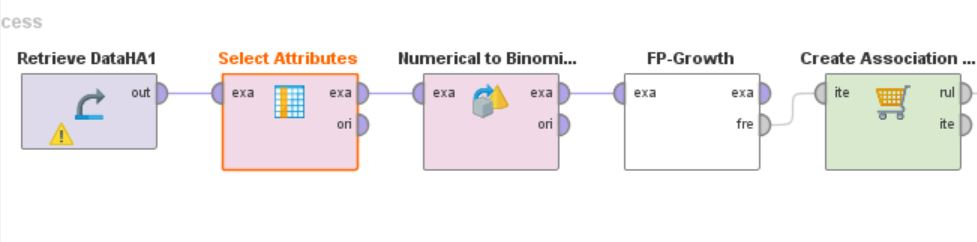
\includegraphics[width=\textwidth]{Question2Process.jpg}

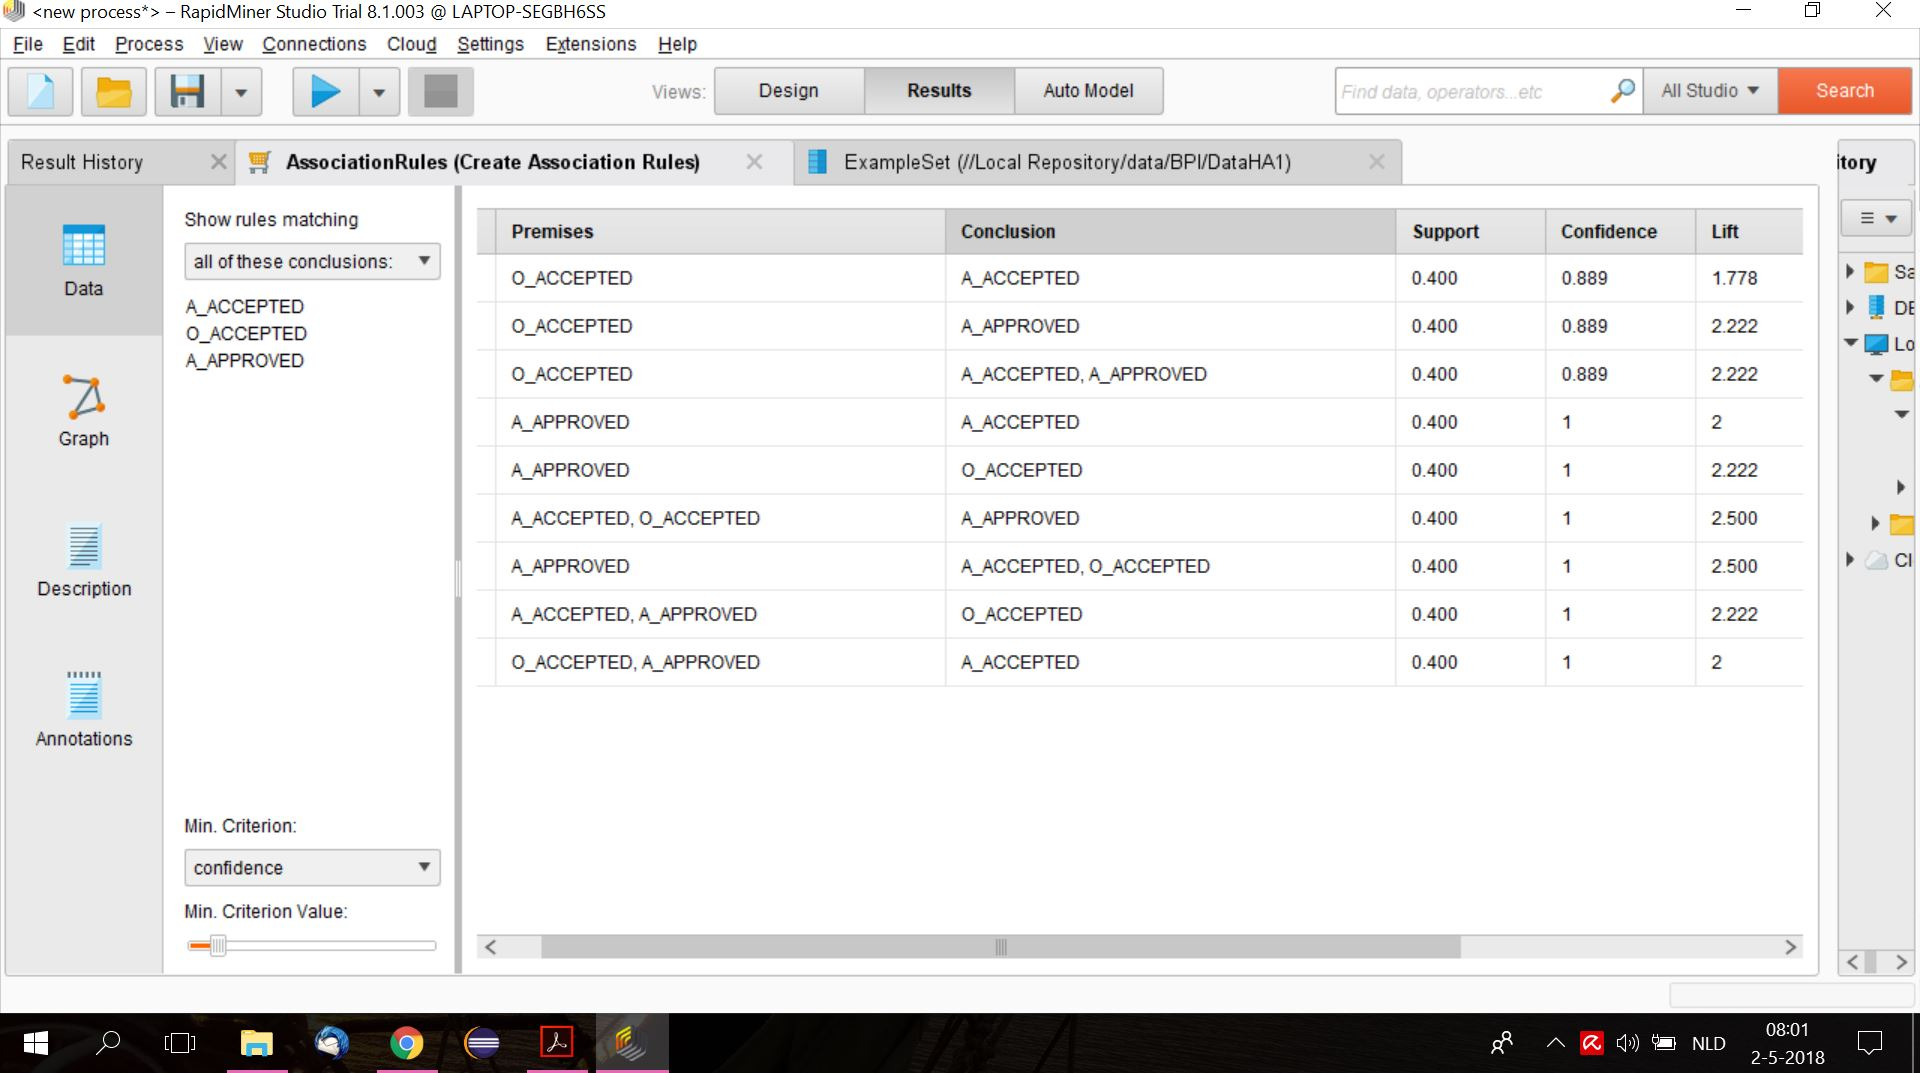
\includegraphics[width=\textwidth]{Question2Rapid.jpg}

I would pick the rule \{A\_ACCEPTED, O\_ACCEPTED\} $\Rightarrow$	\{A\_APPROVED\}
and \{A\_APPROVED\} $\Rightarrow$	\{A\_ACCEPTED, O\_ACCEPTED\}, because they
have the highest lift, confidence and support. When you have a closer look you
will see that the sets are probably of the rules have a back- and forth
relationsip, so they are symmetric. It is an interesting behaviour. Such that
you could summarize it in one rule. 

Then you could look for the next best rules, where lift, support and confidence is the highest.
